\section{Synapsed evaluation}

\begin{frame}{Benchmark preamble}
	The most important part is that synapsed works. We are \textbf{now} able to
	run cached or part of Archipelago in the storage nodes.
	\dspc
	However, let's check its performance.
	\spc
	We will attempt to run most of the previous scenarios using synapsed this 
	time.
	\dspc
	Note, synapsed is proof-of-concept and not performance-tuned. Also, the 
	tested configuration uses a 1Gbit/s connection.
	\note[item]{O κύριως στόχος του synapsed είναι να προσφέρει τη 
		δυνατότητα ή ελαστικότηατα αν το θέλετε, του να τρέχει ο cached 
		ή κομματι του Archipelago σε άλλο κόμβο. Ας δούμε όμως την 
		επίδοσή του
	}
\end{frame}

\begin{frame}{Synapsed results}
	\begin{columns}[t]
		\begin{column}{.5\textwidth}
			Write bandwidth
			\makebox[\textwidth]{
				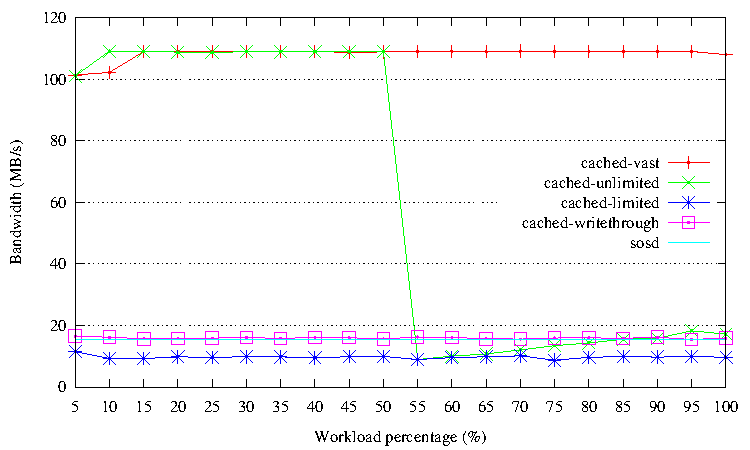
\includegraphics[width=\columnwidth]{images/bw-write-synapsed.pdf}
			}
			Constants:
			\begin{itemize}
				\item cached has 4 threads
				\item workload twice the cache size
				\item block size is 4KB
				\item Parallel requests are 16
			\end{itemize}
		\end{column}
		\begin{column}{.5\textwidth}
			Write latency
			\makebox[\textwidth]{
				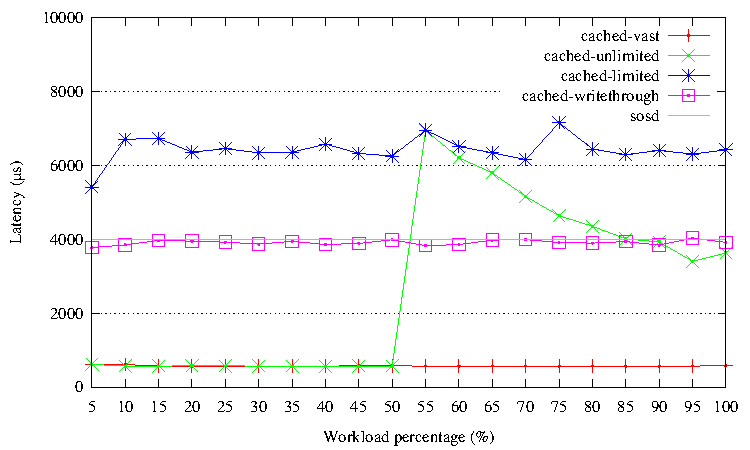
\includegraphics[width=\columnwidth]{images/lat-write-synapsed.pdf}
			}
			Variables:
			\begin{itemize}
				\item cache write policy
				\item maximum cached objects
			\end{itemize}
		\end{column}
	\end{columns}
	\note{Σημεία προσοχής, πρακτικά υπάρχει πολύ μικρή διαφορά με το διάγραμα 
		της σελίδας 32, απλά είναι CAPPED από το δίκτυο. Απλά μπάινει μικρότερο 
		του 1ms latency που για το cached-vast φυσικά κάνει μεγάλη 
		διαφορά.\dspc
		Κατά τα άλλα, το latency αυτό είναι αμελητέο σε σχέση με το 
		τρέχων latency, ενώ αν υπήρχε 10 ή 40Gbit δίκτυο, θα ήταν ακόμα 
		καλύτερα τα πράγματα.
	}
\end{frame}

